\apendice{Documentación técnica de programación}

\section{Introducción}

\section{Estructura de directorios}

\section{Manual del programador}
En esta sección se pretende explicar paso a paso como instalar, compilar y ejecutar el proyecto, como referencia a futuros programadores que usen este proyecto como base para desarrollar nuevas funcionalidades, o nuevos proyectos.
Esos manuales se han desarrollado en un sistema operativo Windows 7 de 64 bits pero también se puede emplear en máquinas de 32 bits.
\section{Instalación, compilación y ejecución del proyecto}

\subsection{Instalación del Entorno.}
	\subsubsection{Java JDK 7}
	Para la ejecución del proyecto, es necesario el uso de Java, por ello se debe realizar una descarga desde la web \cite{java}, eligiendo la versión del sistema operativo en la que ejecutemos el proyecto.En el presente proyecto se ha empleado la versión de Java 7.
	\subsection{NetBeans}
	El servidor, se ha desarrollado bajo el IDE de NetBeans, para instalarlo, se debe ir a la web \cite{netbeans}, y seleccionar la version Java EE(ver figura \ref{fig:netBeansJava}).
	Una vez descargado instalar, y asegurarse de que se selecciona la versión \textbf{GlassFish Server OpenSource Edition}, que instalará de forma automática GlassFish en nuestro ordenador.
	
\imagen{netBeansJava}{Selección de la versión de NetBeans}
	\subsection{Tesseract}
	Para el uso de Tesseract en el servidor, es necesario su instalación, pero \textbf{previamente} se debe instalar el paquete de \textbf{Visual C++ para visual Studio 2013}, que se puede descargar de \cite{paqueteVisual}.Se debe elegir la versión en función de la configuración del sistema operativo siendo:
	\begin{itemize}
		\item \textbf{vcredist\_x64.exe} para la versión de 64 bits.
		\item \textbf{vcredist\_x86.exe} para la versión de 32 bits.
	\end{itemize}
Una vez completada la instalación, se puede proceder a la descarga de Tesseract de \cite{tesseract} donde elegimos el archivo \textbf{tesseract-ocr-setup-3.02.02.exe}(ver figura \ref{fig:tesseractDownload})

\imagen{tesseractDownload}{Selección de descarga Tesseract}
	
	\subsection{Android Studio}
	Para el desarrollo del cliente, se ha utilizado el IDE de Android Studio, para su instalación, se debe ir a la web \cite{androidStudio} y elegir la versión de sistema operativo.
	
	\subsection{Git}
	En el presentre proyecto se ha empleado repositorio Git para el control de versiones, este programa permite clonar el repositio desde BitBucket.Para la instalacion se debe descargar el programa de la web \cite{git} y ejecutar el archivo para proceder a su instalación.

\subsection{Importación del proyecto.}
Para realizar la importación del proyecto se puede realizar de dos maneras, utilizando el CD que se adjunta con la documentación, o clonando el proyecto desde BitBucket

Si se importa desde el CD ir a la sección \ref{cloneServidor} para importar el servidor, o a la sección \ref{cloneCliente} si se desea importar el cliente, por el contrario si se quiere clonar el repositorio seguir leyendo.
\subsubsection{Clonación del proyecto.}

Para clonar el proyecto emplearemos la herramienta de Git que hemos instalado anteriormente. Al abrir la herramienta se nos muestran tres opciones, seleccionamos la opción \textbf{Clone Existing Repository}.
Los datos para poder clonar el repositorio son:
\begin{itemize}
 \item \textbf{Source Location: }\url{https://rober920@bitbucket.org/rober920/miscompras.git}
 \item \textbf{Target Directory: } Directorio donde se desea guardar el repositorio.
\end{itemize}

Al finalizar, el proyecto se descargará en el directorio indicado anteriormente.
\imagen{importGit}{Importación desde Git.}

\subsection{Importación del Servidor.}

Para ejecutar el proyecto del servidor, primero se debe lanzar NetBeans. Para importarlo, seleccionar \textbf{File-Open Project} y buscar el proyecto en la \textbf{Ruta del Proyecto/Servidor}
\imagen{importNetBeans}{Importación del Servidor en NetBeans.}

\cleardoublepage
\subsection{Configuración del Servidor.\label{cloneServidor}}

Antes de ejecutar el proyecto, se deben realizar una serie de configuraciones.
Copiar la carpeta \textbf{resources}(ver figura \ref{fig:carpetaMain}) que se encuentra en la ruta \textbf{ruta del proyecto\textbackslash Servidor\textbackslash misCompras\textbackslash src\textbackslash main} en la carpeta del disco duro \textbf{C:}(ver figura \ref{fig:carpetaC}).

\begin{figure}[ht]
\begin{center} 
\minipage{0.45\textwidth}
  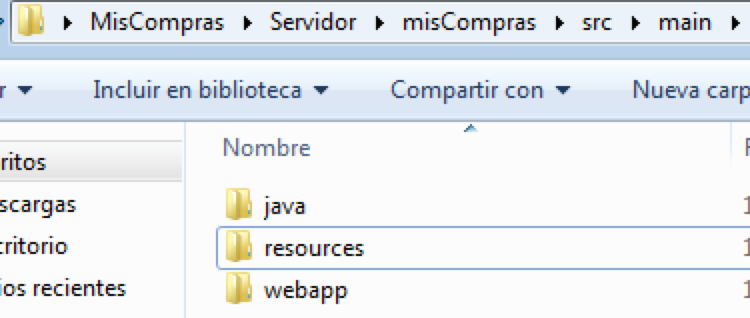
\includegraphics[width=\linewidth]{carpetaMain.png}
  \caption{Carpera resources en el proyecto.}\label{fig:carpetaMain}
\endminipage\hfil
\minipage{0.45\textwidth}
  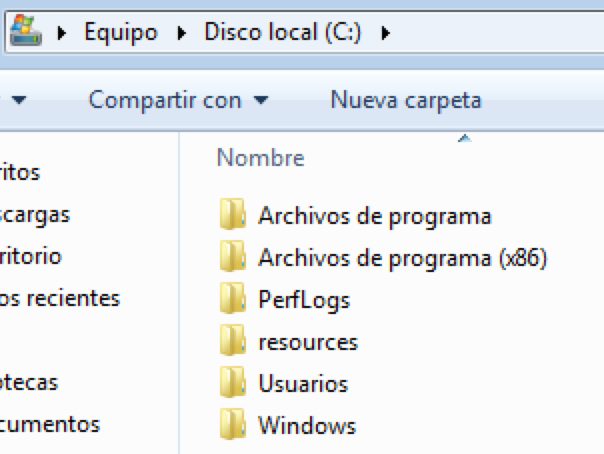
\includegraphics[width=\linewidth]{carpetaC.png}
  \caption{Carpera resources en C:}\label{fig:carpetaC}
\endminipage
\end{center}
\end{figure}



Esta carpeta se empleara para definir OpenCv como una variable de del sistema.
Para esto ir a \textbf{Inicio-Panel de control-Sistema-Opciones avanzadas}, ahí hacer click en \textbf{variables de entorno del sistema}.Para definir una nueva variable hacer click en \textbf{Nuevo}(ver figura \ref{fig:variablesSistema}) y rellenar los campos como(ver figura \ref{fig:variableOpen}):
	\begin{center}
		\textbf{Nombre de la variable} OPENCV
	\end{center}
	y como \textbf{Valor de la variable}
\begin{enumerate}
	\item \textbf{C:/resources/OpenCV\_x64} Si estamos en una maquina de 64 bits.
	\item \textbf{C:/resources/OpenCV\_x86} Si estamos en una maquina de 32 bits.
\end{enumerate}
una ver añadida, añadir al path del sistema como \textbf{\%OPENCV\%}(ver figura \ref{fig:variablePath})

\imagen{variablesSistema}{Nueva variable de sistema}.
\imagen{variableOpen}{Variable de OpenCV.}
\imagen{variablePath}{Variable del path.}

Pulsamos en Aceptar y ya tendríamos definida OpenCV en el path del sistema.

Para terminar se deben copiar los ficheros \textbf{.jar} que se encuentran en \textbf{ruta del proyecto\textbackslash Servidor\textbackslash misCompras\textbackslash src\textbackslash main\textbackslash resources}, estos jar son empleados por Tesseract. Los ficheros se deben pegar en el directorio de instalación de Java \textbf{\textbackslash Java\textbackslash jdk\textbackslash jre\textbackslash lib\textbackslash ext}.
\imagen{configTesseract}{Archivos .jar para Tesseract}

Ya hemos terminado de configurar el proyecto.

Para iniciarlo desde NetBeans pulsamos en el botón de \textbf{Play} que se encuentra en la barra superior del programa.
\imagen{playNetBeans}{Ejecución del proyecto}

Una vez ejecutado se abre el navegador por defecto, y permite comprobar el funcionamiento correcto de la aplicación en el servidor, para ello seleccione un archivo de la carpeta \textbf{tiques} que se encuentra en el proyecto y compruebe el resultado.

\subsection{Importación del Cliente.\label{cloneCliente}}

Para ejecutar el proyecto del cliente, primero se debe lanzar Android Studio. Para importarlo, seleccionar \textbf{Open an existing Android Studio project} y buscar el proyecto en la \textbf{Ruta del Proyecto/Android}. El proceso puede tardar varios minutos.
\imagen{importAndroid}{Importación del Cliente en Android.}

Al terminar la importación puede aparecer un error de que no se encuentra instalada la api 23.0.0 , que es con la que se compilo el proyecto(ver figura \ref{fig:errorAndroid}).Presione en \textbf{Install Build Tools} para inicia la instalación.Una ver terminado comienza la configuración automática del proyecto, este proceso puede tardar varios minutos.
\imagen{errorAndroid}{Error de importación.}

Una vez completado el proyecto esta listo para su ejecución. Se recomienda el uso de un dispositivo físico para la instalación. Para configurar el dipositivo se deben activar las opciones de desarrollo como se puede ver en \cite{debug} y \cite{depuracion}, que explican el proceso.

\subsection{Configuración del Cliente.}

En la la aplicación de Android se ha utilizado OrmLite para la gestión de la Base De datos. Para poder realizar la conversión de Objeto a Tabla de Sqlite , se debe configurar un fichero.El fichero viene por defecto en el proyecto, pero si se desean agregar nuevas clases que se encuentren en la base de datos se debe de crear de nuevo este fichero.
El fichero se crea automáticamente ejecutando la clase \textbf{DataBaseConfig} en el paquete \textbf{model\textbackslash database}.Para ejecutarla ir a \textbf{Run-Edit Configurations..} en la barra de herramientas y añadir una nueva configuración como se ve en la figura \ref{fig:configOrm} pulsamos aceptar y ejecutamos la configuración creada.

\imagen{configOrm}{Configuración OrmLite}
\imagen{configOrm2}{Proceso de configuración OrmLite}

Una vez realizada, OrmLite ya es capaz de mapear nuestro modelo con la base de datos.

\section{Pruebas del sistema}

En el presente trabajo se han desarrollado una batería de pruebas para comprobar la funcionalidad del sistema. Estas pruebas permiten comprobar la validez de este y adaptar el proyecto mas rápidamente  ante nuevos cambios, como por ejemplo añadir nuevas funcionalidades.

\subsection{Pruebas en el cliente.}

Para desarrollar las pruebas en la aplicación de Android se ha empleado Robolectric un framework de test unitarios \cite{robolectric} .

En los pruebas de Android se han testado los interactor, las clases que acceden a la base de datos.
\subsubsection{CaregoryInsertInteractorTest}

\tablaSmall{Test de inserción Categorías}{l c c c c}{test1}
{ \multicolumn{1}{l}{Test} & CategoryInsertTest\\}{ 
Descripción & \begin{tabular}[c]{@{}l@{}}Test que comprueba que se insertan correcta- \\mente categorías en la BD. \end{tabular} \\
Datos de entrada  & \begin{tabular}[c]{@{}l@{}} Categoría(Carne),Categoría(Verduras),\\Categoría(Refrescos)\end{tabular}   \\
Resultados esperados  & True \\
}

\cleardoublepage

\subsubsection{CategoryGetterInteractorTest}

\tablaSmall{Test de obtención de Categorías}{l c c c c}{test2}
{ \multicolumn{1}{l}{Test} & CategoryGetterTest\\}{ 
Descripción & \begin{tabular}[c]{@{}l@{}}Test que comprueba que se obtienen correcta- \\mente categorías de la BD. \end{tabular} \\
Datos de entrada  &  -\\
Resultados esperados  &\begin{tabular}[c]{@{}l@{}} Categoría(Carne),Categoría(Verduras),\\Categoría(Refrescos)\end{tabular}   \\
}

\subsubsection{ProductGetterByCategoryIteratorTest}

\tablaSmall{Test productos por categoría}{l c c c c}{test3}
{ \multicolumn{1}{l}{Test} &  ProductGetterByCategory\\}{ 
Descripción & \begin{tabular}[c]{@{}l@{}}Test que comprueba que se obtienen correcta- \\mente las Lineas de Producto asociadas a una \\Categoría \end{tabular} \\
Datos de entrada  & Categoría(Carne) \\
Resultados esperados  & \begin{tabular}[c]{@{}l@{}}LineaProducto(1,Jamon,1,1.0,1.0) \\LineaProducto(1,Lomo,1,1.0,1.0) \end{tabular} \\
}

\subsubsection{ProductGetterByPriceInteractorTest}

\tablaSmall{Test productos por precio}{l c c c c}{test4}
{ \multicolumn{1}{l}{Test} & CategoryGetterTest\\}{ 
Descripción & \begin{tabular}[c]{@{}l@{}}Test que comprueba que se obtienen correcta- \\mente las Lineas de Producto entre dos \\precios \end{tabular} \\
Datos de entrada  & 1.5,3.5 \\
Resultados esperados  & \begin{tabular}[c]{@{}l@{}}LineaProducto(1,Lomo,1,2.0,2.0) \\LineaProducto(1,Chorizo,2,3.0,6.0) \end{tabular} \\
}

\cleardoublepage

\subsubsection{ProductGetterByTicketInteractorTest}

\tablaSmall{Test productos por tique}{l c c c c}{test5}
{ \multicolumn{1}{l}{Test} &  ProductGetterByTicketTest\\}{ 
Descripción & \begin{tabular}[c]{@{}l@{}}Test que comprueba que se obtienen correcta- \\mente las Lineas de Producto asociadas a un \\Tique \end{tabular} \\
Datos de entrada  & Ticket(1) \\
Resultados esperados  & \begin{tabular}[c]{@{}l@{}}LineaProducto(Ticket(1),Jamón,4,1.0,4.0) \\LineaProducto(Ticket(1),Lomo,2,1.0,2.0) \end{tabular} \\
}

\subsubsection{ProductGetterInteractorTest}

\tablaSmall{Test productos}{l c c c c}{test6}
{ \multicolumn{1}{l}{Test} &  ProductGetterByTicketTest\\}{ 
Descripción & \begin{tabular}[c]{@{}l@{}}Test que comprueba que se obtienen correcta- \\mente todas las Lineas de Producto \end{tabular} \\
Datos de entrada  &  \\
Resultados esperados  & \begin{tabular}[c]{@{}l@{}}LineaProducto(Ticket(1),Jamón,1,1.0,1.0) \\LineaProducto(Ticket(1),Lomo,1,1.0,1.0) \\LineaProducto(Ticket(1),Chorizo,1,1.0,1.0) \\LineaProducto(Ticket(1),Salami,1,1.0,1.0) \end{tabular} \\
}

\subsubsection{ProductGetterIteratorByDateTest}

\tablaSmall{Test productos por fecha}{l c c c c}{test7}
{ \multicolumn{1}{l}{Test} &  ProductGetterByDateTest\\}{ 
Descripción & \begin{tabular}[c]{@{}l@{}}Test que comprueba que se obtienen correcta- \\mente todas las Lineas de Producto entre dos\\fechas \end{tabular}\\
Datos de entrada  &  Date(10-01-2016),Date(11-01-2016)\\
Resultados esperados  & \begin{tabular}[c]{@{}l@{}}LineaProducto(Ticket(1),Jamón,1,1.0,1.0) \\LineaProducto(Ticket(1),Lomo,1,2.0,2.0) \\LineaProducto(Ticket(1),Chorizo,1,3.0,3.0) \\LineaProducto(Ticket(1),Salami,1,4.0,4.0) \end{tabular} \\
}

\subsubsection{ProductGetterIteratorByDateTest}

\tablaSmall{Test productos por fecha}{l c c c c}{test8}
{ \multicolumn{1}{l}{Test} &  ProductGetterByDateTest\\}{ 
Descripción & \begin{tabular}[c]{@{}l@{}}Test que comprueba que se obtienen correcta- \\mente todas las Lineas de Producto entre dos\\fechas \end{tabular}\\
Datos de entrada  &  Date(10-01-2016),Date(11-01-2016)\\
Resultados esperados  & \begin{tabular}[c]{@{}l@{}}LineaProducto(Ticket(1),Jamón,1,1.0,1.0) \\LineaProducto(Ticket(1),Lomo,1,2.0,2.0) \\LineaProducto(Ticket(1),Chorizo,1,3.0,3.0) \\LineaProducto(Ticket(1),Salami,1,4.0,4.0) \end{tabular} \\
}

\subsubsection{ProductInsertIteratorByDateTest}

\tablaSmall{Test inserción de productos}{l c c c c}{test9}
{ \multicolumn{1}{l}{Test} &  ProductInsertTest\\}{ 
Descripción & \begin{tabular}[c]{@{}l@{}}Test que comprueba que se insertan correcta- \\mente lineas de producto en la \\base de datos \end{tabular}\\
Datos de entrada  &  LineaProducto(Ticket(1),Jamón,1,1.0,1.0)\\
Resultados esperados  & True \\
}

\subsubsection{TicketGetterByDateInteractorTest}

\tablaSmall{Test tiques por fecha}{l c c c c}{test10}
{ \multicolumn{1}{l}{Test} &  ProductInsertTest\\}{ 
Descripción & \begin{tabular}[c]{@{}l@{}}Test que comprueba que se obtienen correcta- \\mente los tiques  \\entre dos fechas \end{tabular}\\
Datos de entrada  &  Date(10-01-2016),Date(11-01-2016)\\
Resultados esperados  & Ticket(1)\\
}
\cleardoublepage
\subsubsection{TicketGetterByPriceInteractorTest}

\tablaSmall{Test tiques por importe}{l c c c c}{test11}
{ \multicolumn{1}{l}{Test} &  ProductInsertTest\\}{ 
Descripción & \begin{tabular}[c]{@{}l@{}}Test que comprueba que se obtienen correcta- \\mente los tiques  \\entre dos importes \end{tabular}\\
Datos de entrada  &  11,45\\
Resultados esperados  & Ticket(2),Ticket(3)\\
}

\subsection{Ejecución de Pruebas en el Cliente.}

Para ejecutar las pruebas en la aplciación de Android, primeros debemos cambiar la configuración en las \textbf{Build Variants}, pestaña que se encuentra en el panel lateral izquierdo abajo(ver figura \ref{fig:configTest} ) y seleccionamos UnitTest.

\imagen{configTest}{Configuración de test Android}
\cleardoublepage
Aplicando esta configuración se nos muestran los test para el paquete \textbf{com.ubu.miscompras.model.interactor}

Para ejecutarlos hacemos click derecho sobre el paquete y pulsamos la opción \textbf{Run 'Test in ....'} y esperamos que termine(ver figura \ref{fig:allTest}).
\imagen{runTest}{Ejecutar test en Android}
\imagen{allTest}{Todos Los test ejecutados}

\cleardoublepage

\subsection{Cobertura de Pruebas en el Cliente.}
La cobertura de las pruebas en este caso, es del 80\%(ver figura \ref{fig:coberturaAndroid}), dado que los dos interactors que quedan por testar, dependen de la conexión al servidor, por lo tanto no se han realizado pruebas sobre estas clases.

\imagen{coberturaAndroid}{Cobertura de pruebas Android.}

Para mas información sobre el estado de la cobertura, consultar el CD que se adjunta con este trabajo.

\subsection{Pruebas  del Servidor}

Las pruebas realizadas en el servidor se han realizado bajo el framework de JUnit.

\subsubsection{ImageProccessTest}


\tablaSmall{ITest Lineas de Producto}{l c c c c}{test11}
{ \multicolumn{1}{l}{Test} &  ProductInsertTest\\}{ 
Descripción & \begin{tabular}[c]{@{}l@{}}Test que comprueba que se obtienen correcta- \\mente las lineas de producto de un tique.\end{tabular}\\
Datos de entrada  & Fichero de Imagen   \\
Resultados esperados  & Lista de 8 ficheros. \\
}

\subsubsection{ProductProcessTest}

\tablaSmall{Test espacios y caracteres inválidos}{l c c c c}{test12}
{ \multicolumn{1}{l}{Test} & getTextWithSpacesnTest\\}{ 
Descripción & \begin{tabular}[c]{@{}l@{}}Test que comprueba que se eliminan correcta- \\mente los espacios y caracteres innecesarios de una \\ linea de producto. \end{tabular} \\
Datos de entrada  & 1 . 00 REFRESCOS DE COLA 1, 2O 1 :2O   \\
Resultados esperados  & 1 REFRESCOS DE COLA 1.20 1.20 \\
}

\tablaSmall{Test uso del diccionario}{l c c c c}{test12}
{ \multicolumn{1}{l}{Test} & getTextIncorrectTest()\\}{ 
Descripción & \begin{tabular}[c]{@{}l@{}}Test que comprueba que se corrigen correcta- \\mente el producto de una linea de producto. \end{tabular} \\
Datos de entrada  & 1.00 RER3SCS D3 CAL4 1.20 1.20  \\
Resultados esperados  & 1 REFRESCOS DE COLA 1.20 1.20 \\
}

\tablaSmall{Test archivo csv}{l c c c c}{test12}
{ \multicolumn{1}{l}{Test} & getTextIncorrectTest()\\}{ 
Descripción & \begin{tabular}[c]{@{}l@{}}Test que comprueba que se corrigen correcta- \\mente las cantidades y precios de una\\ linea de producto. \end{tabular} \\
Datos de entrada  & LOO REFRESCOS DE COLA 1.20 l2U  \\
Resultados esperados  & 1 REFRESCOS DE COLA 1.20 1.20 \\
}

\tablaSmall{Test fichero invalido}{l c c c c}{test12}
{ \multicolumn{1}{l}{Test} & getTextNullExceptionTest()\\}{ 
Descripción & \begin{tabular}[c]{@{}l@{}}Test que comprueba que un fichero no puede ser \\null\end{tabular} \\
Datos de entrada  & null  \\
Resultados esperados  & MisComprasException \\
}

\tablaSmall{Test lista invalido}{l c c c c}{test12}
{ \multicolumn{1}{l}{Test} & getTextNullExceptionTest()\\}{ 
Descripción & \begin{tabular}[c]{@{}l@{}}Test que comprueba que una lista\\no puede estar vacia\end{tabular} \\
Datos de entrada  & Lista vacía  \\
Resultados esperados  & MisComprasException \\
}

\tablaSmall{Test salida imagen}{l c c c c}{test12}
{ \multicolumn{1}{l}{Test} & getTextNullExceptionTest()\\}{ 
Descripción & \begin{tabular}[c]{@{}l@{}}Test que comprueba se obtiene correctamente\\el texto de una imagen.\end{tabular} \\
Datos de entrada  & Fichero de imagen  \\
Resultados esperados  & 2 REFRESCOS 1.70 3.40\textbackslash n\textbackslash n\\
}
